
\textbf{\underline{Четвертая глава}} раскрывает детали определения профиля опорной поверхности, на основе информации о точках её касания ногами робота и внутренних датчиков, характеризующих механическое состояние аппарата. Вторая часть главы показывает определение физико-механических свойств опорной поверхности:
жесткости, вязкости и пластичности, и выделение на их основе классов поверхностей на основе информации с датчиков силы, установленных на ногах и внутренних датчиков робота.

\textbf{Первая задача:} имеется поверхность, которой каждому набору координат $x,\ y$ соответствует одно и только одно значение координаты $z$. Необходимо с помощью ощупывания роботом данной поверхности получить плотное облако точек и полигональную сетку. 

Сделано предположение, что расстояние между ногами робота мало относительно размеров поверхности, следовательно поверхность между ногами считается плоскостью.

Для определения геометрических свойств поверхности необходимо получить облако точек касаний опорных поверхностей. То есть мы должны знать трансформацию систем координат от глобальной (к примеру начало движения робота), до конкретного сенсора на ноге. 

Для этого необходимо решить прямую задачу кинематики \pic{fig:StriRus_10_legs_15_angle_v4.png}, \eqref{eq:forw_kin}, а также задачу локализации. Задача локализации в пещере может быть решена с помощью маяков и/или с помощью лидаров/камер. В натурном эксперименте применялись Aruco маркеры.

\begin{figure}[H]
    \centering
     \begin{tikzpicture}
        % Include the image in a node
        \node [above right, inner sep=0] (image) at (0,0) 
        {\centering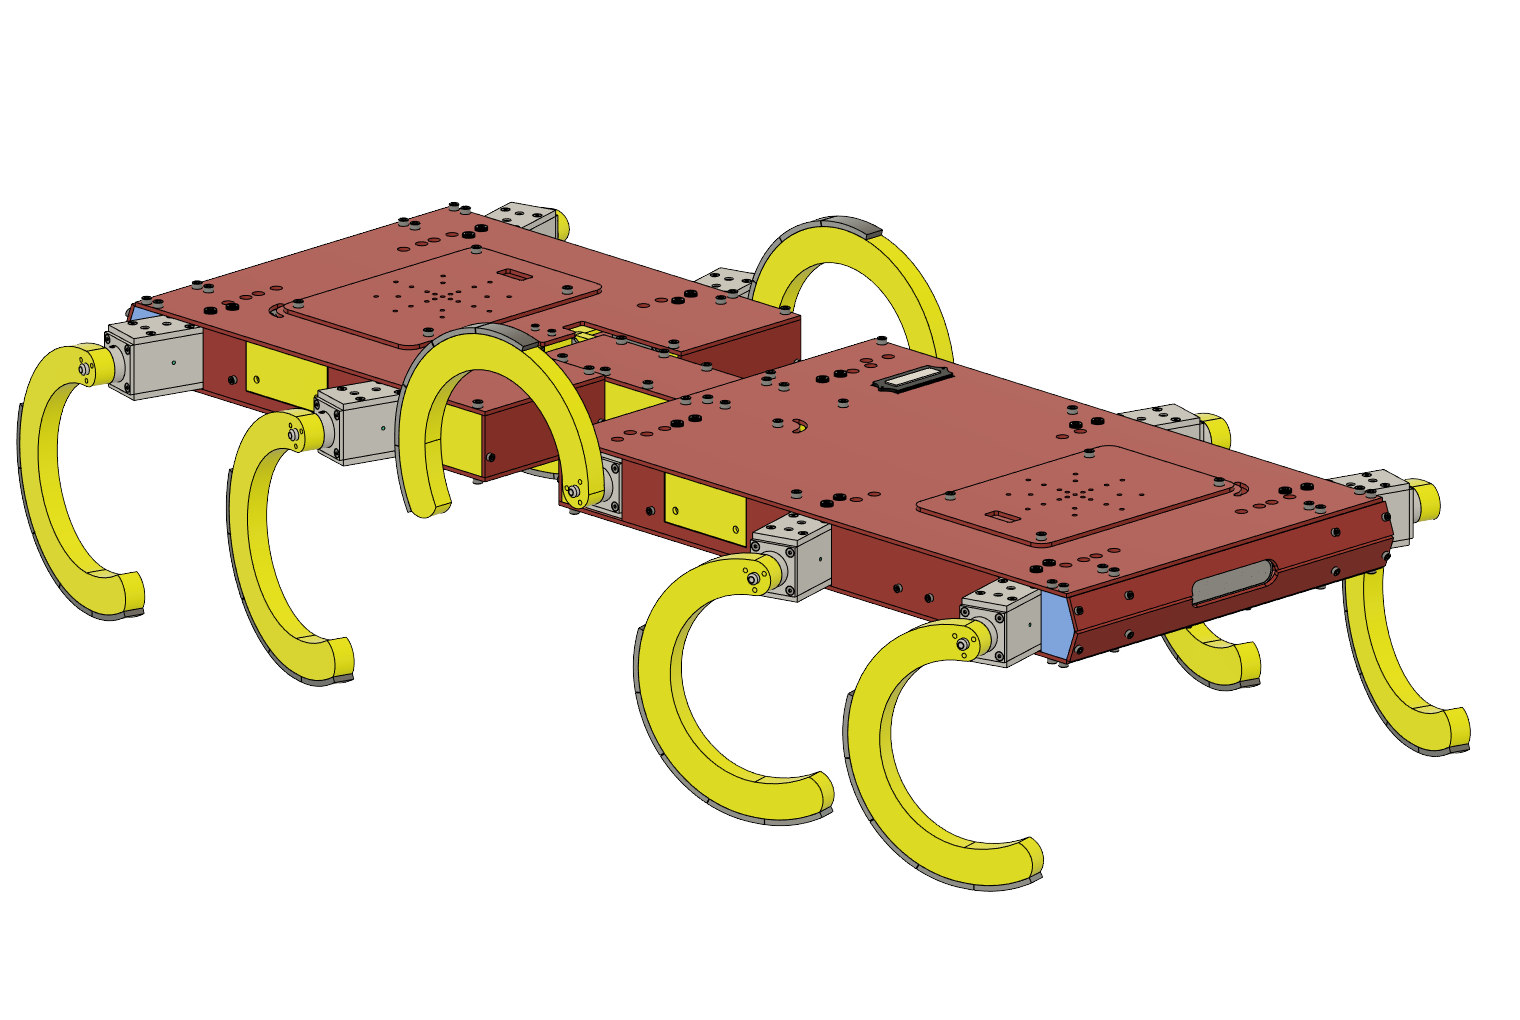
\includegraphics[height=5cm,width=1\textwidth,keepaspectratio]{StriRus_10_legs_15_angle_v4.png}};          
        % Create scope with normalized axes
        \begin{scope}[
            x={($ 0.1*(image.south east)$)},
            y={($ 0.1*(image.north west)$)}]
            % Grid and axes' labels
            % \draw[lightgray,step=1] (image.south west) grid (image.north east);
            % \foreach \x in {0,1,...,10} { \node [below] at (\x,0) {\x}; }
            % \foreach \y in {0,1,...,10} { \node [left] at (0,\y) {\y};}
 
            % Labels

            \coordinate (Xc) at (0.4415/2,-0.2347/2);
            \coordinate (Yc) at (-0.4512/2,-0.2156/2);
            \coordinate (Zc) at (0,0.5/2);
            % Labels
            \tikzstyle{origin} = [rounded corners=2pt, black, fill=gray!40, fill opacity=0.75, text opacity=1, scale=0.8,inner sep=1pt]
            \tikzstyle{transform_text} = [rounded corners=2pt, black, fill=white!85!gray, fill opacity=0.75, text opacity=1, scale=0.8,inner sep=1pt]
            \tikzstyle{transform_arrow} = [thick, green]
    
            % \coordinate (o_g) at (1,9);
            \node[circle,fill=green,scale=0.25] (o_g) at (1,9){};
            \draw[-stealth, very thick,blue] (o_g) -- ++(Xc);
            \draw[-stealth, very thick,green!70!black] (o_g) -- ++(Yc);
            \draw[-stealth, very thick,red] (o_g) -- ++(Zc);
            \node[origin,above right=3pt] at (o_g){\tiny $\mathbf{O_{glob}}$};
    
            % \coordinate (o_b) at (2.9,7.05);
            \node[circle,fill=green,scale=0.25] (o_b) at (2.9,7.05){};
            \draw[-stealth, very thick,blue] (o_b) -- ++(Xc);
            \draw[-stealth, very thick,green!70!black] (o_b) -- ++(Yc);
            \draw[-stealth, very thick,red] (o_b) -- ++(Zc);
            \node[origin,above right=2pt] at (o_b){\tiny $\mathbf{O_{base}}$};
    
            % \coordinate (o_1) at (2.9,6.6);
            \node[circle,fill=green,scale=0.25] (o_1) at (2.9,6.6){};
            \draw[-stealth, very thick,blue] (o_1) -- ++(Xc);
            \draw[-stealth, very thick,green!70!black] (o_1) -- ++(Yc);
            \draw[-stealth, very thick,red] (o_1) -- ++(Zc);
            \node[origin,above right=2pt] at (o_1){\tiny $\mathbf{O_{1}}$};
    
            % \coordinate (o_2) at (4,6);
            \node[circle,fill=green,scale=0.25] (o_2) at (4,6){};
            \draw[-stealth, very thick,blue] (o_2) -- ++(Xc);
            \draw[-stealth, very thick,green!70!black] (o_2) -- ++(Yc)
            node[origin,below=2pt]{\tiny $\mathbf{\alpha_3}$};
            \draw[-stealth, very thick,red] (o_2) -- ++(Zc);
            \node[origin,above right=2pt] at (o_2){\tiny $\mathbf{O_{2}=O_{3}}$};
    
            % \coordinate (o_4) at (7.0,4.55);
            \node[circle,fill=green,scale=0.25] (o_4) at (7.0,4.55){};
            \draw[-stealth, very thick,blue] (o_4) -- ++(Xc);
            \draw[-stealth, very thick,green!70!black] (o_4) -- ++(Yc);
            \draw[-stealth, very thick,red] (o_4) -- ++(Zc);
            \node[origin,above right=2pt] at (o_4){\tiny $\mathbf{O_{4}}$};
    
            % \coordinate (o_5) at (6.7,4.45);
            \node[circle,fill=green,scale=0.25] (o_5) at (6.7,4.45){};
            \draw[-stealth, very thick,blue] (o_5) -- ++(Xc);
            \draw[-stealth, very thick,green!70!black] (o_5) -- ++(Yc);
            \draw[-stealth, very thick,red] (o_5) -- ++(Zc);
            \node[origin,above left=3pt] at (o_5){\tiny $\mathbf{O_{5}=O_{6}}$};
    
            \coordinate (Xcr) at (0.49/2,0.07/2);
            % \coordinate (Ycr) at (-0.38/2,-0.32/2);
            \coordinate (Ycr) at (-0.24/2,-0.43/2);
    
            \draw[-stealth, very thick,blue] (o_5) -- ++(Xcr);
            \draw[-stealth, very thick,green!70!black] (o_5) -- ++(Ycr);
    
    
            % \coordinate (o_7) at (6.36,3.68);
            \node[circle,fill=green,scale=0.25] (o_7) at (6.36,3.68){};
            \draw[-stealth, very thick, blue] (o_7) -- ++(Xcr);
            \draw[-stealth, very thick, green!70!black] (o_7) -- ++(Ycr)
            node[origin,above left=2pt]{\tiny $\mathbf{\alpha_8}$};
            \draw[-stealth, very thick, red] (o_7) -- ++(Zc);
            \node[origin,below right=3pt] at (o_7){\tiny $\mathbf{O_{7}=O_{8}}$};
    
            \node[circle, draw ,fill=green,scale=0.4] (s_1) at (6.6,1.3){1};
            \node[circle,draw, fill=green,scale=0.4] (s_3) at (5.85,1.7){3};
            \node[circle,draw, fill=green,scale=0.4] (s_5) at (5.55,2.9){5};
    
            \draw[-stealth, transform_arrow] (o_g) -- (o_b)
            node[midway,below left=2pt, transform_text]{\tiny $\mathbf{H_{base}^{glob}}$};
    
            \draw[-stealth, transform_arrow] (o_b) -- (o_1)
            node[midway,left=3pt, transform_text]{\tiny $\mathbf{H_{1}^{base}}$};
    
            \draw[-stealth, transform_arrow] (o_1) -- (o_2)
            node[midway,below=2pt, transform_text]{\tiny $\mathbf{H_{2}^{1}}$};
    
            \draw[-stealth, transform_arrow] (o_2) -- (o_4)
            node[midway,below=2pt, transform_text]{\tiny $\mathbf{H_{4}^{3}}$};
    
            \draw[-stealth, transform_arrow] (o_4) -- (o_5)
            node[midway,below right=2pt, transform_text]{\tiny $\mathbf{H_{5}^{4}}$};
    
            \draw[-stealth, transform_arrow] (o_5) -- (o_7)
            node[midway,left=3pt, transform_text]{\tiny $\mathbf{H_{7}^{6}}$};
    
            \draw[-stealth, transform_arrow] (o_7) -- (s_1);
            \draw[-stealth, transform_arrow] (o_7) -- (s_3);
            \draw[-stealth, transform_arrow] (o_7) -- (s_5);
        \end{scope}
    \end{tikzpicture}
    \caption{Кинематическая схема для определения точки касания опорной поверхности роботом}
    \label{fig:StriRus_10_legs_15_angle_v4.png}
\end{figure}

\begin{multline}
    \label{eq:forw_kin}
        H_{leg}^{glob} = H(x_{glob},y_{glob},z_{glob},\alpha_{glob},\beta_{glob},\gamma_{glob})T_z(l_1)\\ T_x(l_2)R_y(\alpha_3)T_x(l_4)T_y(l_5)R_z(-15^{\circ})T_y(l_7)R_y(\alpha_8)
\end{multline}
Где каждая матрица представлены в виде однородной матрицы преобразования $H = \begin{bmatrix}
        \underset{3 \times 3}{R} & \underset{3 \times 1}{T} \\
        \underset{1 \times 3}{0} & \underset{1 \times 1}{1}
    \end{bmatrix}$, где $R_i$ --- матрица поворота, относительно одной из осей, $T_i$ --- вектор сдвига.

Алгоритм получения плотного облака точек следующий. Вначале необходимо очистить оригинальное облако точек от шумов и усреднить близлежащие точки с помощью Voxel grid. Потом из него генерируется полигональная сетка с помощью 2D Триангуляции Делоне \pic{fig:delone_idea.png} (вогнутая оболочка \pic{fig:exp_concave_hull}). На ее основе получается необходимое плотное облако точек \pic{fig:sampled_pcd.png}. 

\begin{figure}[ht!]
    \centering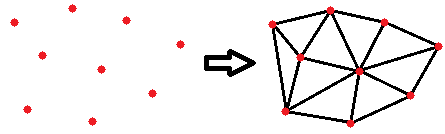
\includegraphics[height=2.5cm,width=1\textwidth,keepaspectratio]{delone_idea.png}
    \caption{2D Триангуляция Делоне (выпуклая оболочка)}
    \label{fig:delone_idea.png}
\end{figure}

На рисунке \ref{fig:exp_concave_hull} проиллюстрирована  важность модификации триангуляции Делоне. Как можно заметить \pic{fig:conv_convex.png} алгоритм построил карту местности там, где робот не ходил и стоит стена. При использовании вогнутой оболочки \pic{fig:conv_concave.png} данная проблема не наблюдается.

\begin{figure}[H]
    \begin{subfigure}[t]{0.32\textwidth}
        \centering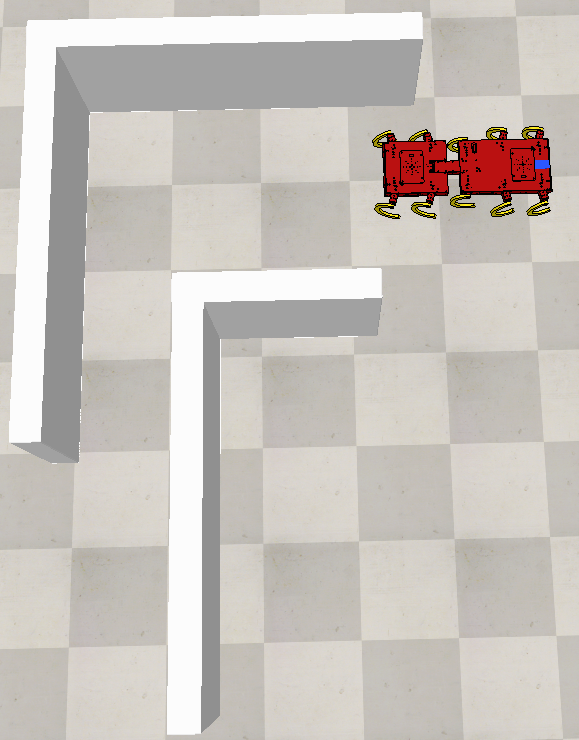
\includegraphics[height=4cm,width=1\textwidth,keepaspectratio]{convex_terr.png}
        \caption{Пример поля}
        \label{fig:convex_terr.png}
    \end{subfigure}
    \begin{subfigure}[t]{0.32\textwidth}
        \centering
        \begin{tikzpicture}
            % Include the image in a node
            \node [above right, inner sep=0] (image) at (0,0)
            {\centering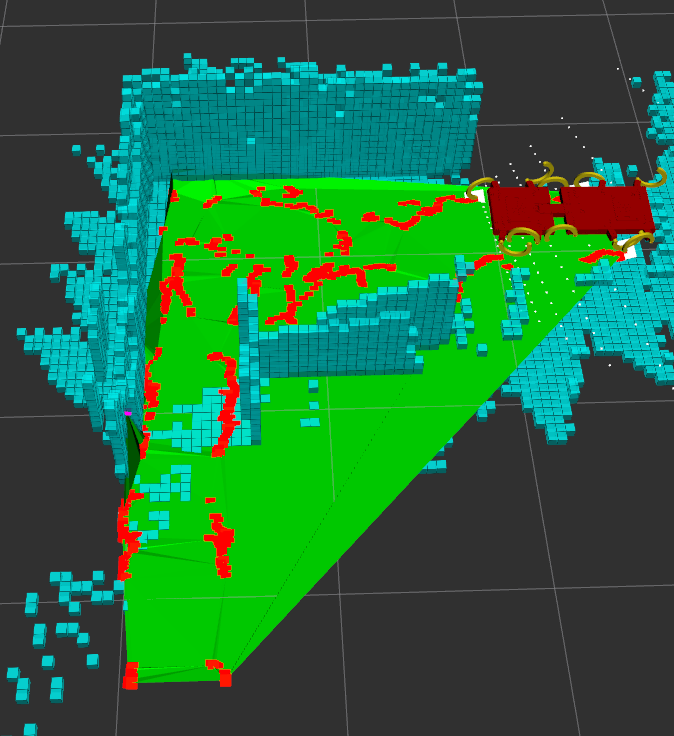
\includegraphics[height=4cm,width=1\textwidth,keepaspectratio]{conv_convex.png}};
            % Create scope with normalized axes
            \begin{scope}[
                x={($ 0.1*(image.south east)$)},
                y={($ 0.1*(image.north west)$)}]
            % Labels
            \draw[stealth-, very thick,green] (5.2,3.5) -- ++(0,-1)
            node[rounded corners=3pt,right,black,fill=white]{\tiny Полученная сетка};

            \draw[stealth-, very thick,green] (5.5,5.5) -- (6.4,4)
            node[rounded corners=3pt,right,black,fill=white]{\tiny Данные лидара};


            \draw[stealth-, very thick,green] (3.4,0.8) -- (5,1);
            \draw[stealth-, very thick,green] (3.4,2.6) -- (5,1)
            node[rounded corners=3pt,right,black,fill=white]{\tiny Следовая дорожка};
        \end{scope}
        \end{tikzpicture}
        \caption{Выпуклая оболочка}
        \label{fig:conv_convex.png}
    \end{subfigure}
    \begin{subfigure}[t]{0.32\textwidth}
        \centering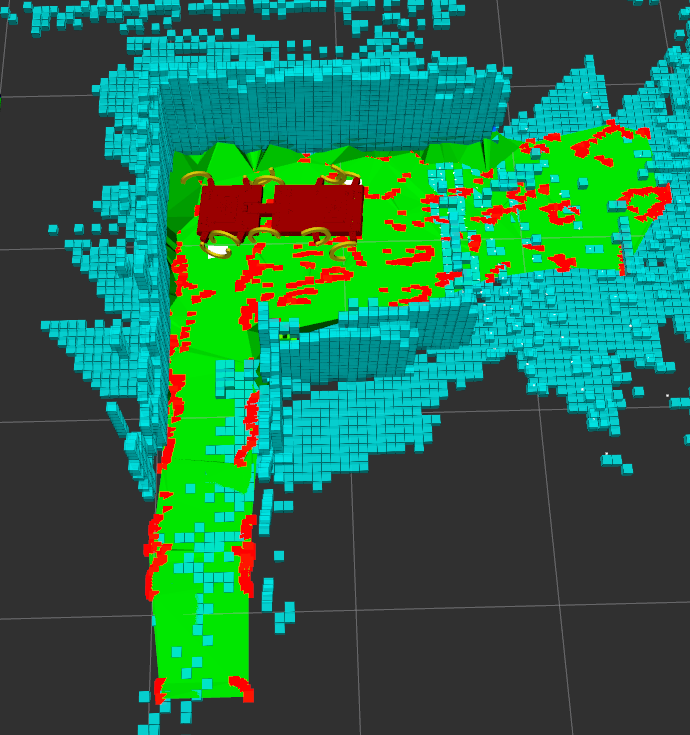
\includegraphics[height=4cm,width=1\textwidth,keepaspectratio]{conv_concave.png}
        \caption{Вогнутая оболочка}
        \label{fig:conv_concave.png}
    \end{subfigure}
    \caption{Объяснение необходимости модификации алгоритма Делоне}
    \label{fig:exp_concave_hull}
\end{figure}

Реализованный алгоритм проверялся, как в симуляции (Рис. \ref{fig:unsolvable_case}), так и на реальном роботе \pic{fig:real_exp_map_creation}.

\begin{figure}[H]
    \begin{subfigure}[t]{0.49\textwidth}
            \centering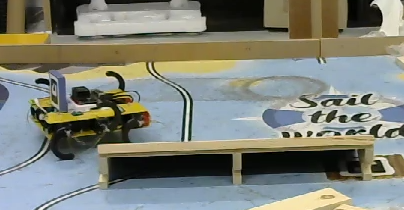
\includegraphics[height=6cm,width=1\textwidth,keepaspectratio]{real_robot_mesh_video_preview.png}
        \caption{Робот проходит препятствие}
        \label{fig:real_robot_mesh_video_preview.png}
    \end{subfigure}
    \begin{subfigure}[t]{0.49\textwidth}
        \centering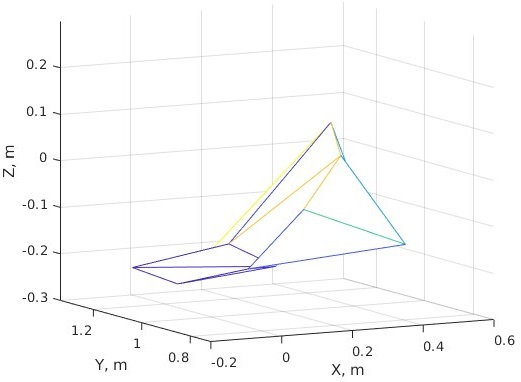
\includegraphics[height=3cm,width=1\textwidth,keepaspectratio]{real_mesh.jpg}
        \caption{Полученная полигональная сетка}
        \label{fig:real_mesh.jpg}
    \end{subfigure}
    \caption{Пример натурного эксперимента}
    \label{fig:real_exp_map_creation}
\end{figure}

Ниже представлены полученные результаты \pic{fig:result_meshes_blah}. Для оценки точности полученных данных использовались метрики C2C \eqref{eqn:hauff} и C2M \pic{fig:metrics}.

\begin{equation}
    \label{eqn:hauff}
    d_{H}(X,\;Y)=\sup _{m\in M}\left\{\,|\mathrm {dist} _{X}(m)-\mathrm {dist} _{Y}(m)|\,\right\}    
\end{equation}
Где $X,\ Y$ непустые подмножества метрического пространства $M$; $\mathrm {dist} _{X}\colon M\to \mathbb {R}$ $\mathrm {dist} _{X}\colon M\to \mathbb {R}$ обозначает функцию расстояния до множества $X$.



\begin{figure}[hp!]
    \begin{center}
    \begin{subfigure}[t]{0.4\textwidth}
        \centering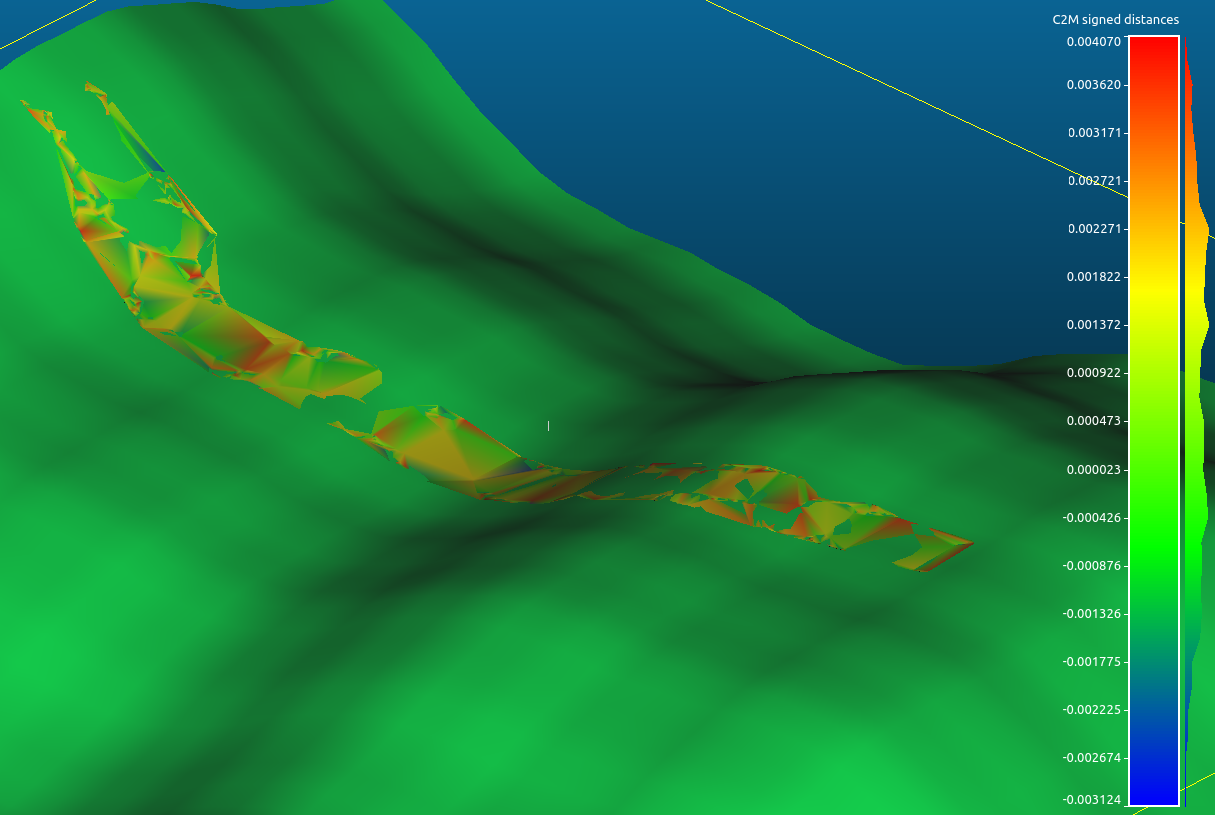
\includegraphics[height=3cm,width=1\textwidth,keepaspectratio]{mesh_comp.png}
        \caption{Наложенные полигональные сетки}
    \end{subfigure}
    \begin{subfigure}[t]{0.59\textwidth}
            \centering
             \begin{tikzpicture}
                % Include the image in a node
                \node [above right, inner sep=0] (image) at (0,0) 
                {\centering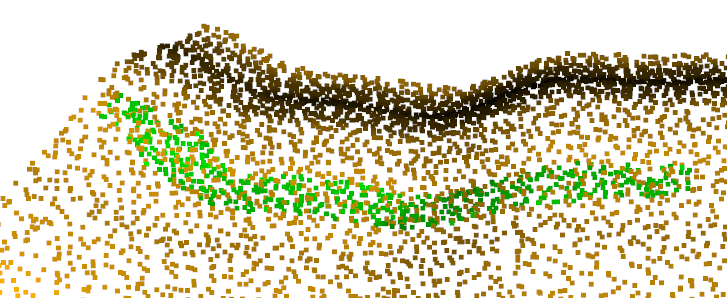
\includegraphics[height=3cm,width=1\textwidth,keepaspectratio]{sampled_pcd.png}};          
                % Create scope with normalized axes
                \begin{scope}[
                    x={($ 0.1*(image.south east)$)},
                    y={($ 0.1*(image.north west)$)}]
                    \draw[stealth-, very thick,green] (3,8) -- (2,8.5);
                    \draw[stealth-, very thick,green] (1,5.5) -- (2,8.5)
                    node[rounded corners=3pt,above,black,fill=white]{\tiny Ground Truth Point Cloud};
         
                    \draw[stealth-, very thick,green] (5.5,3) -- (5.5,8.5)
                    node[rounded corners=3pt,above,black,fill=white]{\tiny Generated Point Cloud};
                \end{scope}
            \end{tikzpicture}
            \caption{Наложенные облака точек}
            \label{fig:sampled_pcd.png}
    \end{subfigure}
    \caption{Результат эксперимента}
    \label{fig:result_meshes_blah}
\end{center}
\end{figure}

\begin{figure}[ht]
    \begin{subfigure}[t]{0.49\textwidth}
        \centering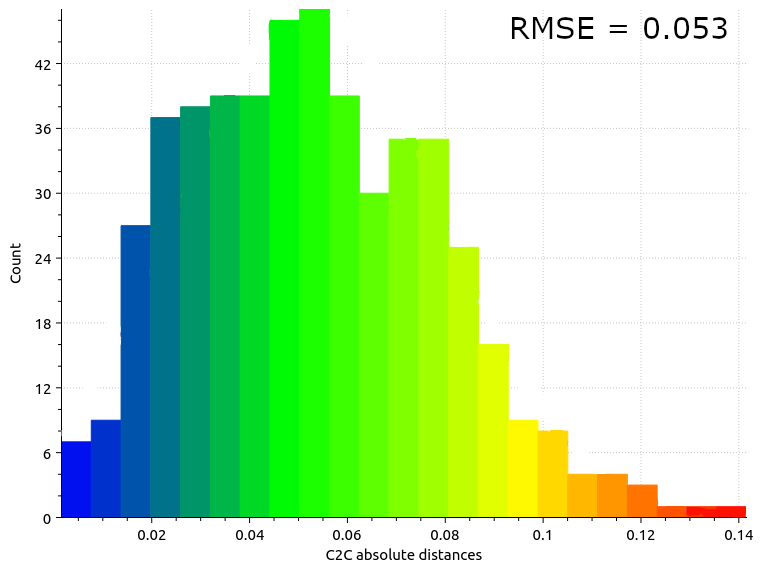
\includegraphics[height=3.5cm,width=1\textwidth,keepaspectratio]{pcd_hist.png}
        \caption{Метрика C2C: гистограмма ошибок (абсолютное расстояние от точки до ближайшей реферальной точки)}
        \label{fig:metric_c2c}
    \end{subfigure}
    \begin{subfigure}[t]{0.49\textwidth}
        \centering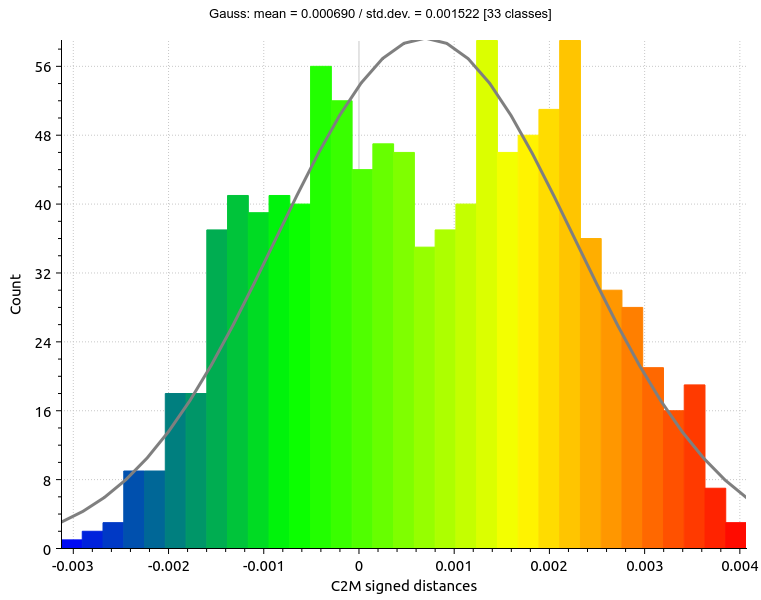
\includegraphics[height=3.5cm,width=1\textwidth,keepaspectratio]{mesh_hist.png}
        \caption{Метрика C2M: Гистограмма ошибок (относительное расстояние от точки до ближайшей реферальной точки)}
        \label{fig:metric_c2m}
    \end{subfigure}
    \caption{Метрики оценки точности полученной карты}
    \label{fig:metrics}
\end{figure}


Как итог, среднеквадратичная ошибка для C2C метрики была в среднем равна 5 см. А для C2M 1 см. В натурном эксперименте среднеквадратичная ошибка по метрике C2C получился 8 см.

\textbf{Вторая задача} это определение физико-механических свойств опорной поверхности. Дана опорная поверхность. Необходимо за минимальное время оценить процентное соотношение твердости, упругости и пластинчатости данной поверхности.

Так как нету абсолютно твердых, упругих и пластинчатых тел, то было решено, что будут выбраны поверхности в которых каждое из свойств доминирует: камень, резина и земля соответственно.

Задачу можно решить следующим образом. Робот идет по поверхности, и собирает данные с датчиков силы и с мотора. На основе предварительного обучения, данные обрабатываются и классифицируется.

Метод опорных векторов (SVM) был выбран  для задачи классификации благодаря ее эффективности и устойчивости при работе с высокоразмерными данными.

Вектор с входными данными представлен следующим образом:
\begin{itemize}
    \item Элемент(1) --- Частота движения ног
    \item (2) --- Пиковая амплитуда давления с датчика силы
    \item (3) --- Ширина давления с датчика силы. Это расстояние между началом и концом акта движения. Такие отрезки складываются и получается ширина.
    \item (4) --- Площадь под кривой силы датчика
    \item (5) --- Пиковая амплитуда крутящего момента двигателя
    \item (6) --- Пиковый крутящий момент двигателя
    \item (7) --- Среднее давление на сенсорах
    \item (8) --- Средняя амплитуда крутящего момента
    \item (9) --- Средний крутящий момент двигателя
    \item (10) --- Ширина крутящего момента двигателя
    \item (11) --- Площадь под кривой крутящего момента двигателя
    \item (12-16) --- Индивидуальная пиковая амплитуда силы такселя 
\end{itemize}

Такой выбор возник благодаря экспериментам и изучению чужих работ. Здесь представлена запись касания ногой на разных поверхностях \pic{fig:s_shape_leg/TaxelIndForce_full.png}. Видно различное поведение сенсоров в зависимости от типа поверхности. 

\begin{figure}[H]
    \centering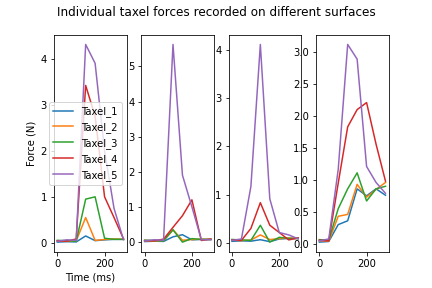
\includegraphics[height=4cm,width=1\textwidth,keepaspectratio]{s_shape_leg/TaxelIndForce.png}
    \caption{Запись активных такселей на разных поверхностях}
    \label{fig:s_shape_leg/TaxelIndForce_full.png}
\end{figure}

Здесь представлены замеры средней линейной скорости движения ноги на разных поверхностях при различных угловых скоростях \pic{fig:s_shape_leg/avg_lin_vel_rev_min.png}. Возможно заметить нелинейную зависимость, что так же может указывать косвенно на тип поверхности.
\begin{figure}[H]
    \centering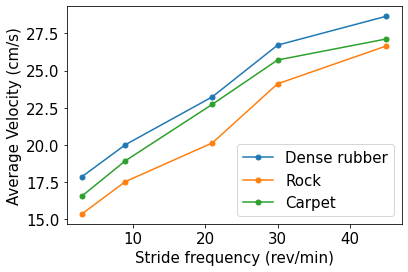
\includegraphics[height=3.5cm,width=1\textwidth,keepaspectratio]{s_shape_leg/avg_lin_vel_rev_min.png}
    \caption{Средняя линейная скорость робота}
    \label{fig:s_shape_leg/avg_lin_vel_rev_min.png}
\end{figure}

В процессе обучения собранные данные были разделены на обучающее (80\% данных) и тестовое множества (20\%). Модель была обучена с использованием ядра на основе функции Пирсона VII (PUK). 

Для оценки эффективности модели использовался тестовый набор. Производительность измерялась с точки зрения точности классификации и F1-score.

Функция принятия решения для SVM-модели \eqref{eq:SVM}:

\begin{align}
    \label{eq:SVM}
    f(x) = w^T x + b
\end{align}

где $x$ --- входной вектор, $w$ является весовым вектором, и $b$ --- смещение.

Универсальное ядро на основе функции Пирсона VII \eqref{eq:PUK}:

\begin{align}
    \label{eq:PUK}
    K(x, y) = (1 + ((||x - y||^2)/\sigma^2)^\omega)^{(-1/\omega)}
\end{align}
Где $x$, $y$ --- векторы во входном пространстве, $||x - y|||$ обозначает евклидово расстояние между $x$ и $y$, $\sigma$ --- масштабный параметр, определяющий "разброс" ядра, $\omega$ --- это параметр формы, который влияет на форму границы принятия решения.

Данные собирались с установки, которая разрабатывалась так, чтобы было возможно быстро сменить тип поверхности, нога робота бесконечно могла совершать движения и узел с ногой был таким же как на реальном роботе \pic{fig:s_shape_leg/s_leg_setup.JPG}.

\begin{figure}[H]
    \begin{subfigure}{0.39\textwidth}
        \centering
        \begin{tikzpicture}
            % Include the image in a node
            \node [above right, inner sep=0] (image) at (0,0)
            {\centering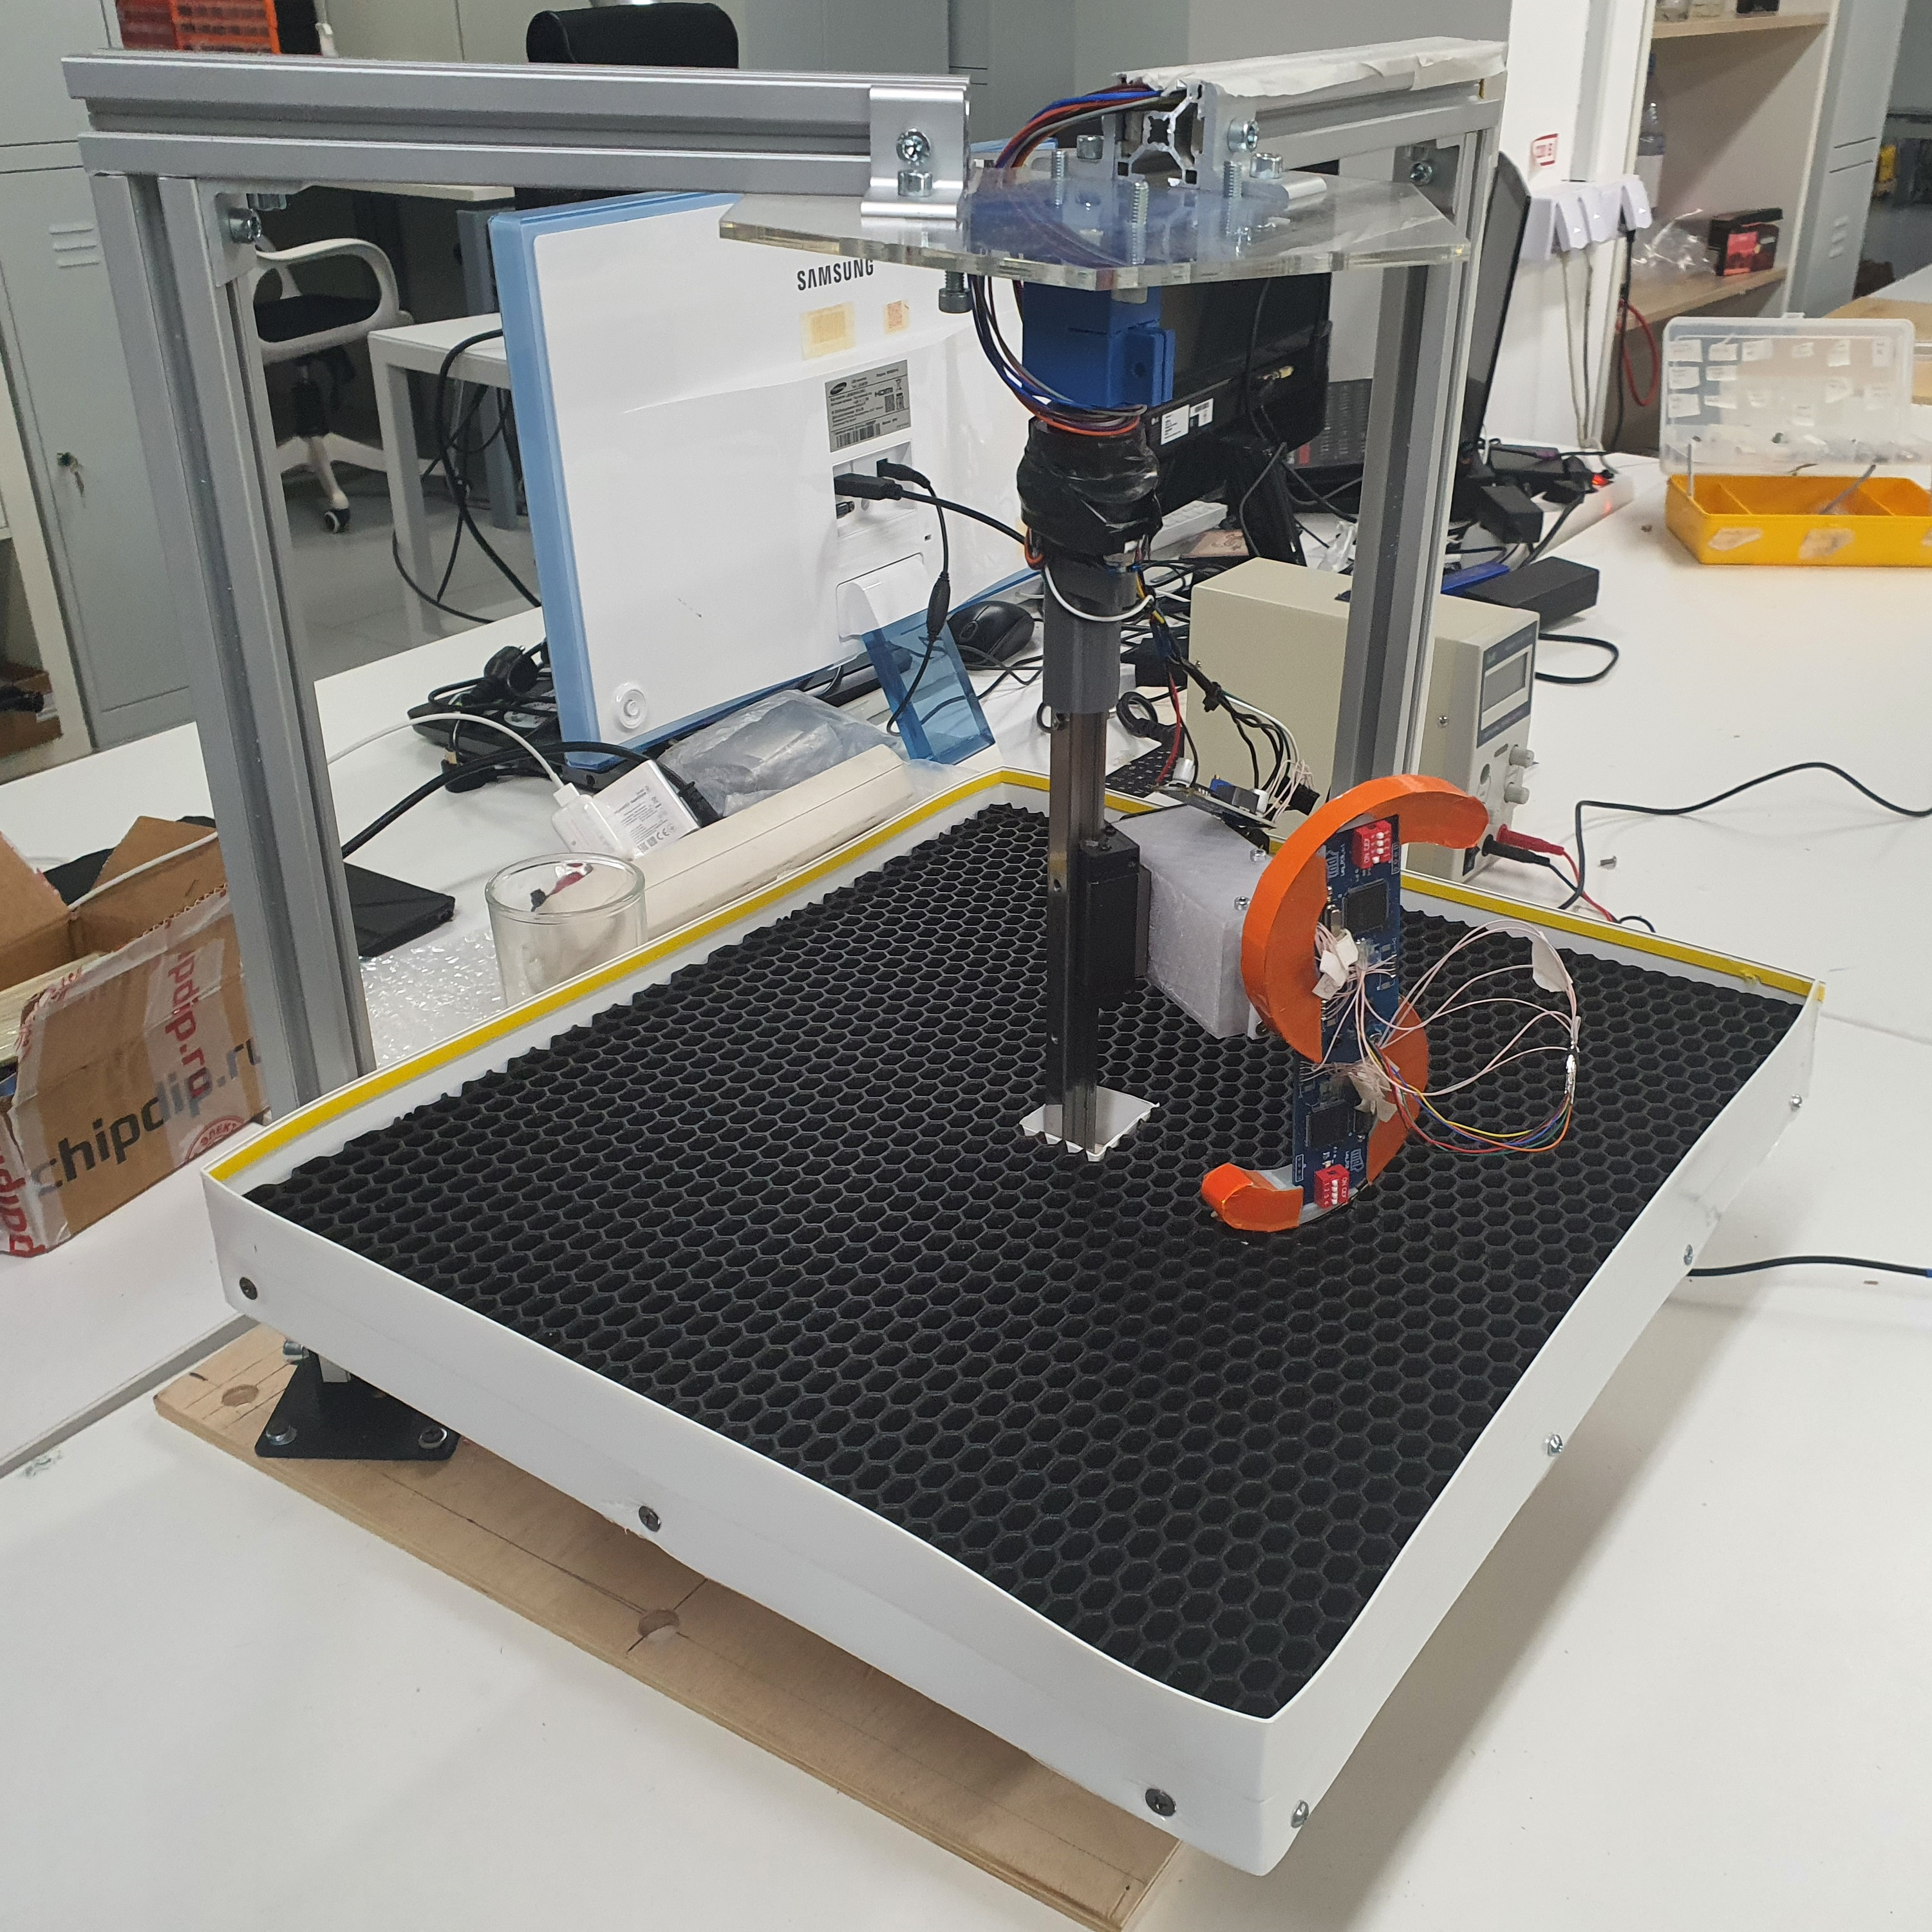
\includegraphics[height=5cm,width=1\textwidth,keepaspectratio]{s_shape_leg/s_leg_setup.JPG}};
            % Create scope with normalized axes
            \begin{scope}[
                x={($ 0.1*(image.south east)$)},
                y={($ 0.1*(image.north west)$)}]
            \draw[stealth-, very thick,green] (3.5,2.5) -- (3,1.5)
            node[rounded corners=3pt,below,black,fill=white]{\tiny Стол для поверхностей};
    
            \draw[stealth-, very thick,green] (7.1,5.4) -- (7.4,7)
            node[rounded corners=3pt,above right,black,fill=white]{\tiny Контроллер};
    
            \draw[very thick,green] (6,6.1) rectangle (8.5,3.5)
            node[above left,black,fill=green]{\tiny S leg};
        \end{scope}
        \end{tikzpicture}
        \caption{Общий вид экспериментальной установки}
    \end{subfigure}
        \begin{subfigure}{0.20\textwidth}
            \centering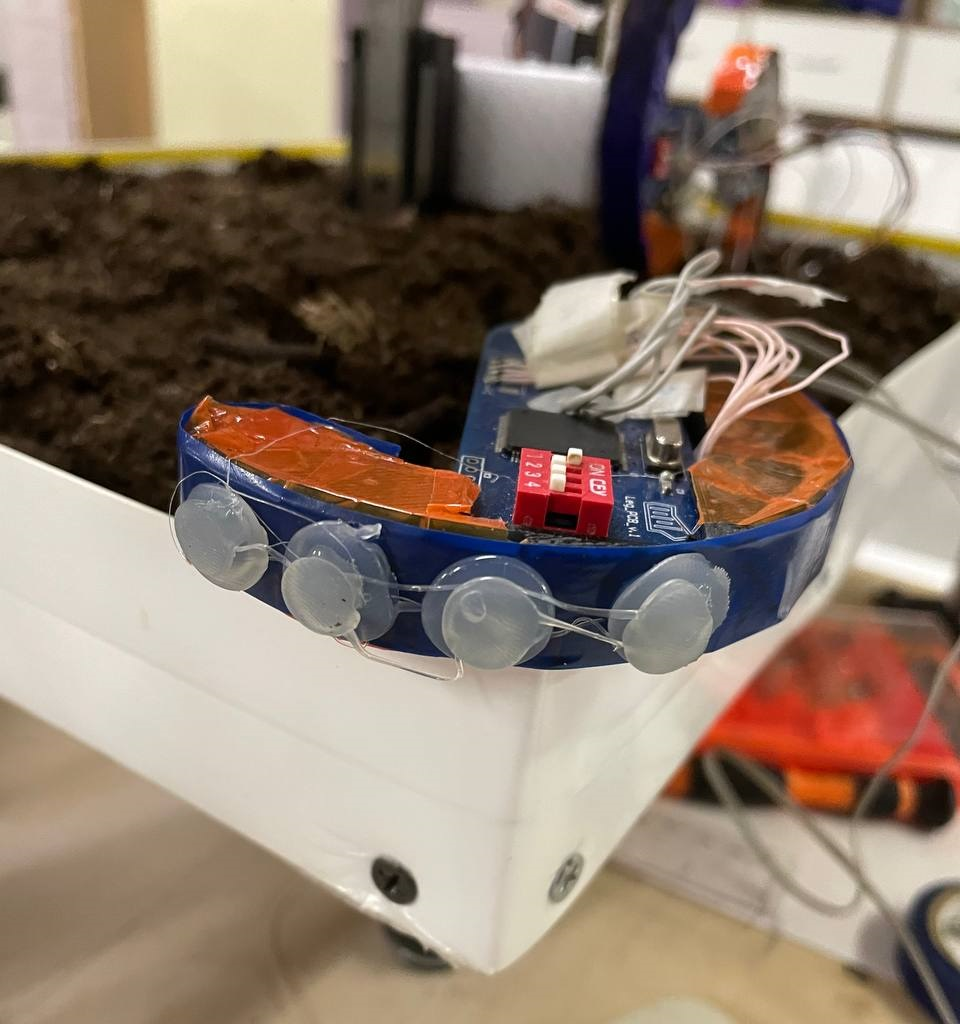
\includegraphics[height=5cm,width=1\textwidth,keepaspectratio]{s_shape_leg/socks_new.jpg}
            \caption{Расположение сенсоров на ноге робота}
            \label{fig:s_shape_leg/socks.jpg}
        \end{subfigure}
        \begin{subfigure}{0.39\textwidth}
            \centering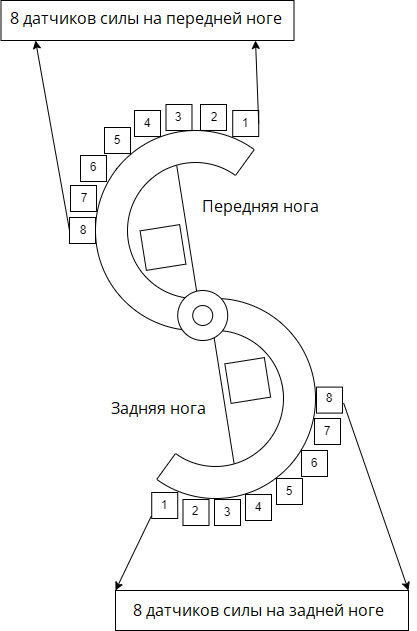
\includegraphics[height=5cm,width=1\textwidth,keepaspectratio]{s_shape_leg/leg_design.png}
            \caption{Схематическое расположение сенсоров на ноге установки}
            \label{fig:s_shape_leg/leg_design.png}
        \end{subfigure}

    \caption{Экспериментальная установка}
    \label{fig:s_shape_leg/s_leg_setup.JPG}
\end{figure}


Результат обучения представлен в виде таблицы \tab{tabular:prob_terrain_classification}.

\begin{table}[H]
    \caption{Вероятность определения типа поверхности}
    \label{tabular:prob_terrain_classification}
    \centering
\begin{tabular}{|c|c|c|c|c|} 
    \cline{3-5}
    \multicolumn{1}{l}{} & \multicolumn{1}{l|}{} & \multicolumn{3}{c|}{\textbf{Предсказанный класс}} \\ 
    \cline{3-5}
    \multicolumn{1}{l}{} &  & Камень & Резина & Земля \\ 
    \hline
    \multirow{3}{*}{{\textbf{Истинный класс}}} & Камень & {\cellcolor[rgb]{0.741,0.843,0.929}}84.0\% & 2.56\% & 13.44\% \\ 
    \hhline{|~----|}
     & Резина & 20.1\% & {\cellcolor[rgb]{0.741,0.843,0.929}}67.8\% & 12.1\% \\ 
    \hhline{|~----|}
     & Земля & 1.0\% & 18.9\% & {\cellcolor[rgb]{0.741,0.843,0.929}}80.1\% \\
    \hline
    \end{tabular}
\end{table}

Она интерпретируется следующим образом. В камне 84\% упругих свойств, 2.56\% упругих и 13.44\% пластинчатых.